\section{Ejemplos}

\noindent El objetivo de esta sección es ejemplificar el uso de los resultados de la sección anterior para obtener distribuciones estacionarias de algunas cadenas de Markov y así estudiar el comportamiento asintótico de las cadenas.

\begin{example}
    Sea $\bm X = \{X_n\}_{n \in \NN}$ una cadena de Markov con espacio de estados $\Ee = \{0, 1, 2, 3, 4\}$ y matriz de transición 
    \[
        P = \begin{pmatrix}
            1/2 & 0 & 0 & 0 & 1/2 \\
            0 & 1/2 & 0 & 1/2 & 0 \\
            0 & 0 & 1 & 0 & 0 \\
            0 & 1/4 & 1/4 & 1/4 & 1/4 \\
            1/2 & 0 & 0 & 0  & 1/2
        \end{pmatrix}.
    \]
    Observemos que los estados $\Ee_T = \{1, 3\}$ son transitorios mientras que los estados $\Ee_R = \{0, 2, 4\}$ son recurrentes; más aún, por ser $\Ee$ finito son recurrentes positivos. Además, $\Cc_1 = \{0,4\}$ y $\Cc_2 = \{2\}$ son clases cerradas e irreducibles. Entonces habrá una distribución estacionaria $\pi^1$ concentrada en $\Cc_1$ y otra $\pi^2$ concentrada en $\Cc_2$. Para obtener $\pi^1$, consideremos la submatriz de transición para $\Cc_1$, dada por 
    \[
        \begin{pmatrix}
            1/2 & 1/2 \\ 1/2 & 1/2
        \end{pmatrix}.
    \]
    La única distribución estacionaria para esta matriz está dada por $\tilde\pi^1 = (1/2, 1/2)$ y, por lo tanto, $\pi^1 = (1/2, 0, 0, 0, 1/2)$. De forma similar, se obtenemos $\pi^2 = (0,0,1,0,0)$, por lo que las distribuciones estacionarias de $\bm X$ están caracterizadas por $\pi^\alpha = (\alpha/2, 0, 1-\alpha, 0, \alpha/2)$ para $\alpha \in [0,1]$.

    Recordemos por otra parte que para cualesquiera $i,j \in \Ee$ se cumplen 
    \[
        \lim_{n \to \infty} \frac{N_j^n}{n} = \frac{1}{m_j} \1_{\{T_j < \infty\}}
    \]
    con probabilidad uno y
    \[
        \lim_{n \to \infty} \frac 1 n \sum_{m = 1}^n P_{ij}^m = \frac{\rho_{ij}}{m_j}.
    \]
    Esto lo podemos usar para estudiar la proporción de pasos que estará una cadena en el estado $j \in \Ee$ si $X_0 = i$, pues en este caso
    \[
        \lim_{n \to \infty} \frac{N_j^n}{n} = \frac{1}{m_j} \1_{\{T_j < \infty, X_0 = i\}}
    \]
    con probabilidad uno. Esto último lo podemos escribir para toda $i \in \Ee$ y toda $j \in \Ee$ mediante el arreglo matricial
    \[
        \begin{pmatrix}
            1/m_0 & 0 & 0 & 0 & 1/m_4 \\
            \1_{\{T_0 < \infty, X_0 = 1\}}/m_0 & 0 & \1_{\{T_2 < \infty, X_0 = 1\}}/m_2 & 0 & \1_{\{T_4 < \infty, X_0 = 1\}}/m_4 \\
            0 & 0 & 1/m_2 & 0 & 0 \\
            \1_{\{T_0 < \infty, X_0 = 3\}}/m_0 & 0 & \1_{\{T_3 < \infty, X_0 = 3\}}/m_2 & 0 & \1_{\{T_4 < \infty, X_0 = 3\}}/m_4 \\
            1/m_0 & 0 & 0 & 0 & 1/m_4 \\
        \end{pmatrix}
    \]
    y por el teorema \ref{teo:distribucion estacionaria reducible}, $m_0 = 1/\pi^1(0)$, $m_2 = 1/\pi^2(2)$ y $m_4 = 1/\pi^1(4)$, de donde la matriz anterior es igual a
    \[
        \begin{pmatrix}
            1/2 & 0 & 0 & 0 & 1/2 \\
            \1_{\{T_0 < \infty, X_0 = 1\}}/2 & 0 & \1_{\{T_2 < \infty, X_0 = 1\}} & 0 & \1_{\{T_4 < \infty, X_0 = 1\}}/2 \\
            0 & 0 & 1 & 0 & 0 \\
            \1_{\{T_0 < \infty, X_0 = 3\}}/2 & 0 & \1_{\{T_3 < \infty, X_0 = 3\}} & 0 & \1_{\{T_4 < \infty, X_0 = 3\}}/2 \\
            1/2 & 0 & 0 & 0 & 1/2
        \end{pmatrix}.
    \]
    Por otra parte, podemos resumir la información que nos da
    \[
        \lim_{n \to \infty} \frac 1 n \sum_{m = 1}^n P_{ij}^m = \frac{\rho_{ij}}{m_j}
    \] para cualesquiera $i, j \in \Ee$ en la siguiente matriz
    \[
        \begin{pmatrix}
            1/2 & 0 & 0 & 0 & 1/2 \\
            \rho_{10}/2 & 0 & \rho_{12} & 0 & \rho_{14}/2 \\
            0 & 0 & 1 & 0 & 0 \\
            \rho_{30}/2 & 0 & \rho_{32} & 0 & \rho_{34}/2 \\
            1/2 & 0 & 0 & 0 & 1/2
        \end{pmatrix},
    \] por lo que basta encontrar $\rho_{10}, \rho_{12}, \rho_{14}, \rho_{30}, \rho_{32}$ y $\rho_{34}$ para obtener todos los límites explícitamente. Para obtener estos valores, podemos obtener  $\rho_{\Cc_1}(1), \rho_{\Cc_1}(3), \rho_{\Cc_2}(1)$ y $\rho_{\Cc_2}(3)$ pues si entramos a una clase cerrada, casi seguramente visitaremos todos los estados en la clase. Más aún, como solamente hay dos clases cerradas, $\rho_{\Cc_1}(1) = 1 - \rho_{\Cc_2}(1)$ y $\rho_{\Cc_1}(3) = 1 - \rho_{\Cc_2}(3)$, entonces bastará resolver el sistema de ecuaiones 
    \begin{align*}
        \rho_{\Cc_1}(1) & = \frac 1 2 \rho_{\Cc_1}(1) + \frac 1 2 \rho_{\Cc_1}(3), \\
        \rho_{\Cc_1}(3) & = \frac 1 4 \rho_{\Cc_1}(1) + \frac 1 4 \rho_{\Cc_1}(3) + \frac 1 4,
    \end{align*}
    de donde $\rho_{\Cc_1}(1) = \rho_{\Cc_1}(3) = 1/2$ y, por lo tanto,
    \[
        \begin{pmatrix}
            1/2 & 0 & 0 & 0 & 1/2 \\
            \rho_{10}/2 & 0 & \rho_{12} & 0 & \rho_{14}/2 \\
            0 & 0 & 1 & 0 & 0 \\
            \rho_{30}/2 & 0 & \rho_{32} & 0 & \rho_{34}/2 \\
            1/2 & 0 & 0 & 0 & 1/2
        \end{pmatrix} = 
        \begin{pmatrix}
            1/2 & 0 & 0 & 0 & 1/2 \\
            1/4 & 0 & 1/2 & 0 & 1/4 \\
            0 & 0 & 1 & 0 & 0 \\
            1/4 & 0 & 1/2 & 0 & 1/4 \\
            1/2 & 0 & 0 & 0 & 1/2
        \end{pmatrix}.
    \]
    De esta forma hemos obtenido el comportamiento asintótico de la cadena dependiendo del estado en el que comience la cadena $\bm X$.
\end{example}

\begin{example} \label{ej:nym infinita}
    Consiremos que $\bm X = \{X_n\}_{n \in \NN}$ es una cadena de nacimiento y muerte en $\NN$ irreducible, es decir que $p_i := P_{i,i+1} > 0$ para $i \in \NN$ y $q_i := P_{i,i-1}$ para $i \geq 1$. Denotemos además $r_i = P_{ii}$ para toda $i \in \NN$. Para obtener una distribución estacionaria $\pi$, se debe satisfacer $\pi = \pi P$, que nos da el sistema de ecuaciones
    \begin{align*}
        \pi(0) & = \pi(0) r_0 + \pi(1) q_1, \\
        \pi(i) & = \pi(i-1) p_{i-1} + \pi(i) r_i + \pi(i+1) q_{i+1} \quad \text{ para } i \geq 1.
    \end{align*}
    De $1 - r_i = p_i + q_i$, el sistema de ecuaciones anterior se reduce a 
    \begin{align*}
        q_1 \pi(1) - p_0 \pi(0)  & = 0, \\
        q_{i+1} \pi(i+1) - p_i \pi(i) & = q_i \pi(i) - p_{i-1} \pi(i-1) \quad \text{ para } i \geq 1.
    \end{align*}
    De un argumento inductivo se sigue que 
    \[
        q_{i+1} \pi(i+1) - p_i \pi(i) = 0 
    \] para toda $i \in \NN$ y entonces 
    \[
        \pi(i+1) = \frac{p_i}{q_{i+1}} \pi(i)    
    \]
    es cierto para toda $i \in \NN$. Al definir 
    \[
        \eta_i = \frac{\prod_{j = 0}^{i-1} p_j }{ \prod_{j = 1}^i q_j },    
    \] donde el producto vacío es uno, tendremos de forma recursiva que $\pi(i) = \eta_i \pi(0)$ para toda $i \in \NN$. Si $\sum_{i = 0}^\infty \eta_i < \infty$, la cadena de nacimiento y muerte tiene una distribución estacionaria $\pi$ dada por 
    \[
        \pi(i) = \frac{\eta_i}{\sum_{j = 0}^\infty \eta_j}
    \]
    para toda $i \in \NN$, que además es única por ser una $\bm X$ irreducible. Como la cadena es irreducible y existe una distribución estacionaria cuando $\sum_{i = 0}^\infty \eta_i < \infty$, vemos que una condición necesaria y suficiente para que la cadena de nacimiento y muerte sea recurrente positiva es que 
    \[
        \sum_{i = 0}^\infty \frac{\prod_{j = 0}^{i-1} p_j }{ \prod_{j = 1}^i q_j } < \infty.
    \] En la primera parte de cadenas de Markov, se vio que
    \[
        \sum_{i = 0}^\infty \frac{\prod_{j = 1}^i q_j }{ \prod_{j = 0}^{i-1} p_j } < \infty
    \] es condición necesaria y suficiente para que una cadena de nacimiento y muerte irreducible sea transitoria. Así pues, la cadena de nacimiento y muerte será recurrente nula si y sólo si 
    \[
        \sum_{i = 0}^\infty \frac{\prod_{j = 0}^{i-1} p_j }{ \prod_{j = 1}^i q_j } = \infty \quad \text{ y } \quad \sum_{i = 0}^\infty \frac{\prod_{j = 1}^i q_j }{ \prod_{j = 0}^{i-1} p_j } = \infty.
    \]
    Así las cosas, hemos logrado clasificar todas las cadenas de nacimiento y muerte irreducibles en transitorias, recurrentes positivas y recurrentes nulas.
\end{example}

\begin{example} \label{ej:nym finito}
    Supongamos que $\bm X = \{X_n\}_{n \in \NN}$ es una cadena de nacimiento y muerte irreducible en $\Ee = \{0, 1, \ldots, d\}$, con $d \geq 1$. Siguiendo un procedimiento similar al del ejemplo \ref{ej:nym infinita}, la cadena tendrá una única distribución estacionaria $\pi$ dada por 
    \[
        \pi(i) = \frac{\eta_i}{\sum_{j = 0}^d \eta_j},
    \] donde 
    \[
        \eta_i = \frac{\prod_{j = 0}^{i-1} p_j}{\prod_{j = 1}^i q_j}.    
    \]
\end{example}

\begin{example}
    Consideremos el modelo de difusión de Bernoulli--Laplace con $6$ partículas, que es una cadena de Markov $\bm X$ con espacio de estados $\Ee = \{0,1,2,3\}$ y matriz de transición
    \[
        P = \begin{pmatrix}
            0 & 1 & 0 & 0 \\
            1/9 & 4/9 & 4/9 & 0 \\
            0 & 4/9 & 4/9 & 1/9 \\
            0 & 0 & 1 & 0
        \end{pmatrix}.
    \]
    Esta cadena resulta ser una cadena de nacimiento y muerte. Por el ejemplo \ref{ej:nym finito}, $\eta_0 = 1$ y
    \[
        \eta_1 = \frac{1}{\frac 1 9} = 9, \quad \eta_2 = \frac{1 \times \frac 4 9}{\frac 1 9 \times \frac 4 9} = 9 \quad \text{ y } \quad \eta_3 = \frac{1 \times \frac 4 9 \times \frac 1 9}{\frac 1 9 \times \frac 4 9 \times 1} = 1,
    \] de donde la única distribución única está dada por 
    \[
        \pi = \left( \frac 1 {20}, \frac 9 {20}, \frac 9 {20}, \frac 1 {20} \right).
    \]
\end{example}

\begin{example}
    Consideremos ahora una modificación de la cadena de Ehrenfest con 4 bolas etiquetadas del 1 al 4. Supongamos que inicialmente algunas bolas están en la urna 1 y el resto se encuentra en la urna 2. Se selecciona una entero de $\{1, 2, 3, 4\}$ y se saca la bola etiquetada con tal entero de la urna en la que se encuente, para después seleccionar de forma equiprobable a qué urna se meterá la bola. Si denotamos por $X_n$ al número de bolas en la urna 1 después del $n$-ésimo experimento, $\bm X = \{X_n\}_{n \in \NN}$ es una cadena de Markov con espacio de estados $\Ee = \{0,1, 2, 3, 4\}$ y matriz de transición
    \[
        P = \begin{pmatrix}
            1/2 & 1/2 & 0 & 0 & 0 \\
            1/8 & 1/2 & 3/8 & 0 & 0 \\
            0 & 1/4 & 1/2 & 1/4 & 0 \\
            0 & 0 & 3/8 & 1/2 & 1/8 \\
            0 & 0 & 0 & 1/2 & 1/2
        \end{pmatrix}.
    \] Notemos que nuevamente tendremos una cadena de nacimiento y muerte irreducible. Siguiendo el ejemplo \ref{ej:nym finito}, su única distribución estacionaria estará dada por
    \[
        \pi = \left( \frac 1{16}, \frac 1 4, \frac 3 8, \frac 1 4, \frac 1{16} \right).
    \]
\end{example}

\begin{example}
    Consideremos una cadena de rachas con probabilidad $0 < p < 1$, es decir $\bm X = \{X_n\}_{n \in \NN}$ es una cadena de Markov con espacio de estados $\NN$ y probabilidades de transición $P_{i,i+1} = 1 - P_{i0} = p$. Es claro que esta cadena es irreducible y además 
    \[
        m_0 = \EE[T_0 \,\vert\, X_0 = 0] =  \frac{p}{1-p} < \infty,
    \]
    por lo que la cadena es recurrente positiva. Así, debe tener una única distribución estacionaria $\pi$. De $\pi = \pi P$ obtenemos el sistema de ecuaciones,
    \begin{align*}
        \pi(0) & = \sum_{i = 0}^\infty (1-p) \pi(i), \\
        \pi(i) & =  p \pi(i-1) \quad \text{ para } i \geq 1.
    \end{align*}
    Como $\sum_{i = 0}^\infty \pi(i) = 1$, se deduce que $\pi(i) = p^i (1-p)$ para toda $i \in \NN$.
\end{example}

\begin{example}
    Supongamos que una partícula se mueve sobre los vértices de un cubo de la siguiente manera: en cada paso la partícula se mueve a cualquier vértice adyacente al que se encuentre, que se escoge de forma equiprobable, independientemente de su trayectoria pasada. Sea $I$ el vértice inicial y $O$ el vértice opuesto a $I$. Vamos a calcular las siguientes cantidades:
    \begin{enumerate}
        \item El número esperado de pasos para regresar a $I$.
        \item El número esperado de visitas a $O$ antes de regresar a $I$.
        \item El número esperado de pasos para visitar $O$ por primera vez.
    \end{enumerate}
    Denotemos por $A$ al conjunto de vértices adyacentes a $I$ y por $B$ al conjunto de vértices adyacentes a $O$. Si $X_n$ es la posición de la partícula después del $n$-ésimo movimiento, $\bm X = \{X_n\}_{n \in \NN}$ es una cadena de Markov con espacio de estados $\Ee = \{I, A, B, O\}$ y matriz de transición $P$ dada por
    \[
        \bordermatrix{
            & I & A & B & O \cr
            I & 0 & 1 & 0 & 0 \cr
            A & 1/3 & 0 & 2/3 & 0 \cr
            B & 0 & 2/3 & 0 & 1/3 \cr
            O & 0 & 0 & 1 & 0
        }.
    \] Por lo tanto tenemos una cadena de nacimiento y muerte irreducible con distribución estacionaria 
    \[
        \pi = \left(\frac 1 8, \frac 3 8, \frac 3 8, \frac 1 8\right).
    \]
    Recordando que $m_j = 1/\pi(j)$, la solución de (1) está dada por $m_I = 8$. Para (2), estamos buscando $\gamma_O^I$. Recordemos que $\gamma^I$ es una medida invariante con $\gamma_I^I = 1$ tal que $\gamma^I \leq \mu$ para cualquier otra medida invariante $\mu$ con $\mu(I) = 1$. De hecho, por ser $\bm X$ irreducible, la desigualdad es igualdad. Notemos que $\mu = 8\pi$ es una medida invariante tal que $\mu(I) = 1$ y, por lo tanto, $\gamma_O^I = 8 \pi(O) = 1$. Finalmente buscamos $\EE[T_O \,\vert\, X_0 = I]$, para lo que basta resolver el sistema de ecuaciones
    \begin{align*}
        \EE[T_O \,\vert\, X_0 = I] & = \EE[T_O \,\vert\, X_0 = A] + 1, \\
        \EE[T_O \,\vert\, X_0 = A] & = \frac 1 3 \EE[T_O \,\vert\, X_0 = I] + \frac 2 3 \EE[T_O \,\vert\, X_0 = B] + 1 \\
        \EE[T_O \,\vert\, X_0 = B] & = \frac 2 3 \EE[T_O \,\vert\, X_0 = I] + 1,
    \end{align*}
    de donde $\EE[T_O \,\vert\, X_O = I] = 10$.
\end{example}

Para poder entender los siguientes ejemplos, necesitamos un par de definiciones nuevas, además de un resultado auxiliar.

\begin{definition}
    Sea $\bm X$ una cadena de Markov con espacio de estados $\Ee$ y matriz de transición $P$. Diremos que $\bm X$, o bien la matriz $P$, es \emph{doblemente estocástica} si 
    \[
        \sum_{i \in \Ee} P_{ij} = 1    
    \]
    se satisface para toda $j \in \Ee$.
\end{definition}

\begin{definition}
    Sean $\bm X$ una cadena de Markov con espacio de estados $\Ee$ y matriz de transición $P$, además de $\pi$ una medida, \emph{i.e.} $\pi: \Ee \to \RR$ con $\pi(i) \geq 0$ para todo estado $i \in \Ee$. Diremos que $\pi$ y $\bm X$ están en \emph{balance detallado} si para cualesquiera $i, j \in \Ee$ se cumple que 
    \[
        \pi(i) P_{ij} = \pi(j) P_{ji}.    
    \]
\end{definition}

\begin{proposition}
    Si $\bm X$ y $\pi$ están en balance detallado entonces $\pi$ es una medida invariante para $\bm X$.
\end{proposition}

\begin{proof}
    Para cada $j \in \Ee$,
    \[
        \sum_{i \in \Ee} \pi(i) P_{ij} = \sum_{i \in \Ee} \pi(j) P_{ji} = \pi(j). \qedhere
    \]
\end{proof}

\begin{example}
    Si $\bm X$ es una cadena de Markov irreducible, con espacio de estados $\Ee$ finito y doblemente estocástica, entonces tiene una única distribución estacionaria $\pi$, donde \[\pi(j) = \frac 1 K,\] con $K$ la cardinalidad de $\Ee$.
\end{example}

\begin{example}
    Un crupier se encuentra aburrido porque no llegan jugadores a su mesa de blackjack, por lo que se pone a barajar una baraja de 52 cartas repetidamente. De tan aburrido que está se hace la pregunta de cuántas veces deberá barajar los naipes para regresar al orden original bajo dos esquemas:
    \begin{enumerate}
        \item Baraja todo el mazo de cartas y cualquier orden de las cartas es equiprobable como resultado.
        \item Saca una carta al azar y la coloca en una posición distinta a la original, escogida de forma equiprobable.
    \end{enumerate}
    Consideremos que $X_n$ es el orden de la baraja después de la $n$-ésima barajada y denotemos por $\bm X = \{X_n\}_{n \in \NN}$ la cadena de Markov que se obtiene, con espacio de estados $\Ee$ dado por los posibles ordenamientos de los naipes. Observemos que si existe un barajeo que lleve del estado $i$ al estado $j$, ese mismo barajeo llevará de un estado $k$ al estado $j$, de donde el $j$-ésimo renglón de la matriz $P$ asociada a $\bm X$ es la $j$-ésima columna en un orden distinto, por lo que $\bm X$ es una cadena doblemente estocástica. Así pues, en promedio se requerirán $52!$ barajeos, bajo cualquiera de los esquemas, para regresar al orden en el que se encontraba la baraja de cartas inicialmente.
\end{example}

\begin{example}[Caminata aleatoria sobre gráficas] \label{ej:caminatas sobre graficas}
    Una gráfica es un par $G = (V, E)$ de conjuntos tal que $E \subset [V]^2$, donde $[V]^k = \{A \subset V : \abs{A} = k\}$; esto es, los elementos de $E$, llamados aristas, son subconjuntos de dos elementos de $V$, llamados vértices. Diremos que $i \in V$ y $j \in V$ son vecinos si $\{i, j\} \in E$. Para $i, j \in V$ diremos que podemos ir de $i$ a $j$ si existen elementos $i_0, i_1, \ldots, i_n \in V$, con $i_0 = i$ y $j = i_n$ tales que $\{i_{k-1}, i_k\} \in E$ para $k \in \{1, \ldots, n\}$. La gráfica será conexa si para cualesquiera $i, j \in V$, se puede ir de $i$ a $j$. Además se define la valencia $v_i$ de $i \in V$ como la cantidad de vecinos que tiene $i$, \emph{i.e.} $v_i = \abs{\{e \in E : i \in e\}}$.

    Definimos una caminata aleatoria sobre una gráfica $G$ conexa, con $V$ finito de cardinalidad al menos 2, de la siguiente manera: si nos encontramos en $i \in V$, iremos a cualquiera de sus vecinos de forma equiprobable, independientemente de la trayectoria pasada. Así, si $X_n$ es el vértice después del $n$-ésimo movimiento, tendremos que $\bm X = \{X_n\}_{n \in \NN}$ es una cadena de Markov irreducible con espacio de estados $V$ y probabilidades de transición
    \[
        P_{ij} = \begin{cases}
            \frac 1 {v_i} & \text{ si } \{i, j\} \in E, \\
            0 & \text{ en otro caso}.
        \end{cases}    
    \]
    Entonces $\mu = \{v_i : i \in V\}$ es una medida que está en balance detallado con $\bm X$. En efecto $0 < v_i \leq \abs V - 1 < \infty$ y para cualesquiera $i, j \in V$,
    \[
        \mu(i) P_{ij} = v_i \frac 1 {v_i} = 1 = v_j \frac 1 {v_j} = \mu(j) P_{ji}   
    \] si $\{i,j\} \in E$ y 
    \[
        \mu(i) P_{ij} = \mu(j) P_{ji} = 0
    \] en otro caso. Ahora observemos que $0 < \sum_{i \in V} v_i \leq \abs E \leq \binom{\abs V}{2} < \infty$ y, por lo tanto, si definimos $\pi$ por
    \[
        \pi(i) = \frac{v_i}{\sum_{j \in V} v_j},
    \]
    obtendremos la única distribución estacionaria de la cadena.
\end{example}

\begin{example}
    Consideremos un caballo en un tablero de ajedrez que comienza en una esquina y se mueve aleatoriamente de la siguiente manera: puede ir, de forma equiprobable, a cualquier casilla que le sea permitido bajo su movimiento en L, ver la figura \ref{fig:caballitos}, y nos preguntamos cuántos movimientos tardará en promedio el caballo en regresar a la esquina de la que comenzó. Así, los movimientos aleatorios del caballo forman una caminata aleatoria sobre una gráfica conexa y finita. 

    De la figura \ref{fig:caballitos}, vemos que hay 4 vértices de valencia 2, 8 vértices de valencia 3, 20 vértices de valencia 4, 16 vértices de valencia 6 y 16 vértices de valencia 8. Luego, por el ejemplo \ref{ej:caminatas sobre graficas}, si denotamos por $c$ la esquina en la que comenzó el caballo y por $X_n$ su posición tras el $n$-ésimo movimiento,
    \[
        \EE[T_c \,\vert\, X_0 = c] = \frac 1 {\pi(c)} = \frac{\sum_{i \in V} v_i}{v_c} = \frac{8 + 24 + 80 + 96 + 128}{2} = 168.
    \]
    Es decir que el caballo tardará en promedio 168 movimientos en regresar a la esquina en la que comenzó.

    \begin{figure}[ht]
        \centering
        \begin{subfigure}[b]{0.3\textwidth}
            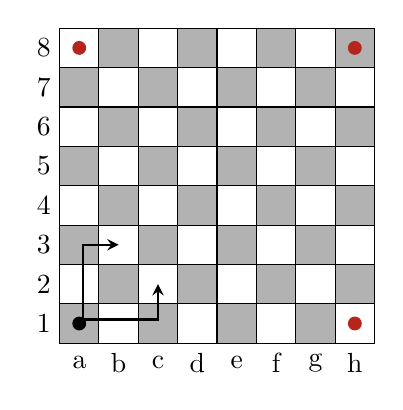
\begin{tikzpicture}[x=5mm,y=5mm]
                \draw[fill=black!30,even odd rule] (0,0) 
                foreach \n in {1,2,3,4} { -- ++ (8,0) -- ++ (0,1) -- ++ (-8,0) -- ++ (0,1) } -- (8,8)
            
                foreach \n in {1,2,3,4} { -- ++ (0,-8) -- ++ (-1,0) -- ++ (0,8) -- ++ (-1,0) } -- cycle
            
                foreach[count=\n] \m in {a,b,...,h} { (-0.4,\n-0.5) node {\n} (\n-0.5,-0.5) node {\m} };

                \fill (0.5,0.5) circle[radius=2.5pt];
                \fill[BrickRed] (7.5,0.5) circle[radius=2.5pt];
                \fill[BrickRed] (0.5,7.5) circle[radius=2.5pt];
                \fill[BrickRed] (7.5,7.5) circle[radius=2.5pt];
                \draw[-stealth, thick] (0.6,0.6) -- (0.6,2.5) -- (1.5,2.5);
                \draw[-stealth, thick] (0.6,0.6) -- (2.5,0.6) -- (2.5,1.5);
            \end{tikzpicture}
        \end{subfigure} ~
        \begin{subfigure}[b]{0.3\textwidth}
            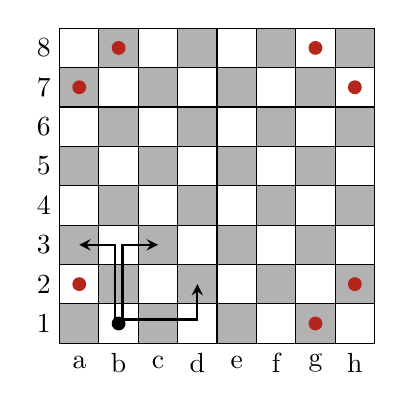
\begin{tikzpicture}[x=5mm,y=5mm]
                \draw[fill=black!30,even odd rule] (0,0) 
                foreach \n in {1,2,3,4} { -- ++ (8,0) -- ++ (0,1) -- ++ (-8,0) -- ++ (0,1) } -- (8,8)
            
                foreach \n in {1,2,3,4} { -- ++ (0,-8) -- ++ (-1,0) -- ++ (0,8) -- ++ (-1,0) } -- cycle
            
                foreach[count=\n] \m in {a,b,...,h} { (-0.4,\n-0.5) node {\n} (\n-0.5,-0.5) node {\m} };

                
                \fill (1.5,0.5) circle[radius=2.5pt];
                \fill[BrickRed] (0.5,1.5) circle[radius=2.5pt];
                \fill[BrickRed] (0.5,6.5) circle[radius=2.5pt];
                \fill[BrickRed] (1.5,7.5) circle[radius=2.5pt];
                \fill[BrickRed] (6.5,0.5) circle[radius=2.5pt];
                \fill[BrickRed] (7.5,1.5) circle[radius=2.5pt];
                \fill[BrickRed] (6.5,7.5) circle[radius=2.5pt];
                \fill[BrickRed] (7.5,6.5) circle[radius=2.5pt];
                \draw[-stealth, thick] (1.4,0.6) -- (1.4,2.5) -- (0.5,2.5);
                \draw[-stealth, thick] (1.6,0.6) -- (1.6,2.5) -- (2.5,2.5);
                \draw[-stealth, thick] (1.6,0.6) -- (3.5,0.6) -- (3.5,1.5);
            \end{tikzpicture}
        \end{subfigure} ~
        \begin{subfigure}[b]{0.3\textwidth}
            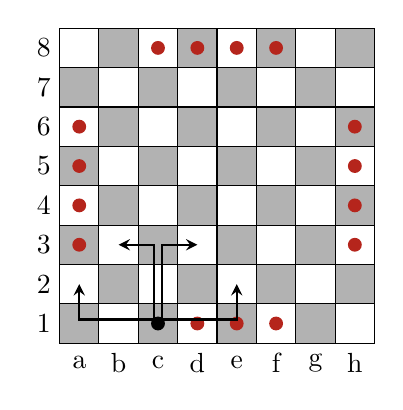
\begin{tikzpicture}[x=5mm,y=5mm]
                \draw[fill=black!30,even odd rule] (0,0) 
                foreach \n in {1,2,3,4} { -- ++ (8,0) -- ++ (0,1) -- ++ (-8,0) -- ++ (0,1) } -- (8,8)
            
                foreach \n in {1,2,3,4} { -- ++ (0,-8) -- ++ (-1,0) -- ++ (0,8) -- ++ (-1,0) } -- cycle
            
                foreach[count=\n] \m in {a,b,...,h} { (-0.4,\n-0.5) node {\n} (\n-0.5,-0.5) node {\m} };

                \fill (2.5,0.5) circle[radius=2.5pt];
                \fill[BrickRed] (3.5,0.5) circle[radius=2.5pt];
                \fill[BrickRed] (4.5,0.5) circle[radius=2.5pt];
                \fill[BrickRed] (5.5,0.5) circle[radius=2.5pt];
                \fill[BrickRed] (2.5,7.5) circle[radius=2.5pt];
                \fill[BrickRed] (3.5,7.5) circle[radius=2.5pt];
                \fill[BrickRed] (4.5,7.5) circle[radius=2.5pt];
                \fill[BrickRed] (5.5,7.5) circle[radius=2.5pt];
                \fill[BrickRed] (0.5,2.5) circle[radius=2.5pt];
                \fill[BrickRed] (0.5,3.5) circle[radius=2.5pt];
                \fill[BrickRed] (0.5,4.5) circle[radius=2.5pt];
                \fill[BrickRed] (0.5,5.5) circle[radius=2.5pt];
                \fill[BrickRed] (7.5,2.5) circle[radius=2.5pt];
                \fill[BrickRed] (7.5,3.5) circle[radius=2.5pt];
                \fill[BrickRed] (7.5,4.5) circle[radius=2.5pt];
                \fill[BrickRed] (7.5,5.5) circle[radius=2.5pt];
                \draw[-stealth, thick] (2.4,0.6) -- (2.4,2.5) -- (1.5,2.5);
                \draw[-stealth, thick] (2.6,0.6) -- (2.6,2.5) -- (3.5,2.5);
                \draw[-stealth, thick] (2.6,0.6) -- (4.5,0.6) -- (4.5,1.5);
                \draw[-stealth, thick] (2.4,0.6) -- (0.5,0.6) -- (0.5,1.5);
            \end{tikzpicture}
        \end{subfigure}

        \begin{subfigure}[b]{0.3\textwidth}
            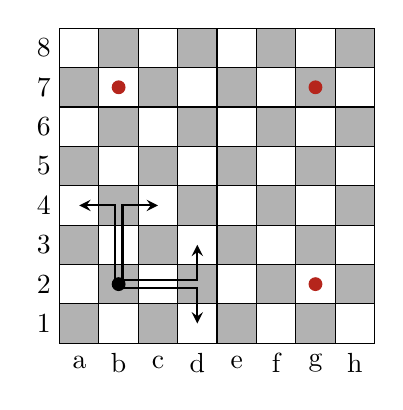
\begin{tikzpicture}[x=5mm,y=5mm]
                \draw[fill=black!30,even odd rule] (0,0) 
                foreach \n in {1,2,3,4} { -- ++ (8,0) -- ++ (0,1) -- ++ (-8,0) -- ++ (0,1) } -- (8,8)
            
                foreach \n in {1,2,3,4} { -- ++ (0,-8) -- ++ (-1,0) -- ++ (0,8) -- ++ (-1,0) } -- cycle
            
                foreach[count=\n] \m in {a,b,...,h} { (-0.4,\n-0.5) node {\n} (\n-0.5,-0.5) node {\m} };

                \fill (1.5,1.5) circle[radius=2.5pt];
                \fill[BrickRed] (1.5,6.5) circle[radius=2.5pt];
                \fill[BrickRed] (6.5,1.5) circle[radius=2.5pt];
                \fill[BrickRed] (6.5,6.5) circle[radius=2.5pt];
                \draw[-stealth, thick] (1.4,1.6) -- (1.4,3.5) -- (0.5,3.5);
                \draw[-stealth, thick] (1.6,1.6) -- (1.6,3.5) -- (2.5,3.5);
                \draw[-stealth, thick] (1.6,1.6) -- (3.5,1.6) -- (3.5,2.5);
                \draw[-stealth, thick] (1.6,1.4) -- (3.5,1.4) -- (3.5,0.5);
            \end{tikzpicture}
        \end{subfigure} ~
        \begin{subfigure}[b]{0.3\textwidth}
            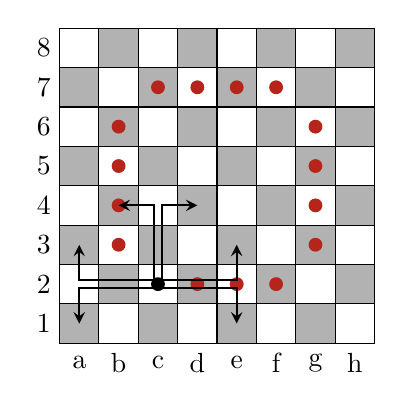
\begin{tikzpicture}[x=5mm,y=5mm]
                \draw[fill=black!30,even odd rule] (0,0) 
                foreach \n in {1,2,3,4} { -- ++ (8,0) -- ++ (0,1) -- ++ (-8,0) -- ++ (0,1) } -- (8,8)
            
                foreach \n in {1,2,3,4} { -- ++ (0,-8) -- ++ (-1,0) -- ++ (0,8) -- ++ (-1,0) } -- cycle
            
                foreach[count=\n] \m in {a,b,...,h} { (-0.4,\n-0.5) node {\n} (\n-0.5,-0.5) node {\m} };

                \fill (2.5,1.5) circle[radius=2.5pt];
                \fill[BrickRed] (3.5,1.5) circle[radius=2.5pt];
                \fill[BrickRed] (4.5,1.5) circle[radius=2.5pt];
                \fill[BrickRed] (5.5,1.5) circle[radius=2.5pt];
                \fill[BrickRed] (2.5,6.5) circle[radius=2.5pt];
                \fill[BrickRed] (3.5,6.5) circle[radius=2.5pt];
                \fill[BrickRed] (4.5,6.5) circle[radius=2.5pt];
                \fill[BrickRed] (5.5,6.5) circle[radius=2.5pt];
                \fill[BrickRed] (1.5,2.5) circle[radius=2.5pt];
                \fill[BrickRed] (1.5,3.5) circle[radius=2.5pt];
                \fill[BrickRed] (1.5,4.5) circle[radius=2.5pt];
                \fill[BrickRed] (1.5,5.5) circle[radius=2.5pt];
                \fill[BrickRed] (6.5,2.5) circle[radius=2.5pt];
                \fill[BrickRed] (6.5,3.5) circle[radius=2.5pt];
                \fill[BrickRed] (6.5,4.5) circle[radius=2.5pt];
                \fill[BrickRed] (6.5,5.5) circle[radius=2.5pt];
                \draw[-stealth, thick] (2.4,1.6) -- (2.4,3.5) -- (1.5,3.5);
                \draw[-stealth, thick] (2.6,1.6) -- (2.6,3.5) -- (3.5,3.5);
                \draw[-stealth, thick] (2.6,1.6) -- (4.5,1.6) -- (4.5,2.5);
                \draw[-stealth, thick] (2.6,1.4) -- (4.5,1.4) -- (4.5,0.5);
                \draw[-stealth, thick] (2.4,1.6) -- (0.5,1.6) -- (0.5,2.5);
                \draw[-stealth, thick] (2.4,1.4) -- (0.5,1.4) -- (0.5,0.5);
            \end{tikzpicture}
        \end{subfigure} ~
        \begin{subfigure}[b]{0.3\textwidth}
            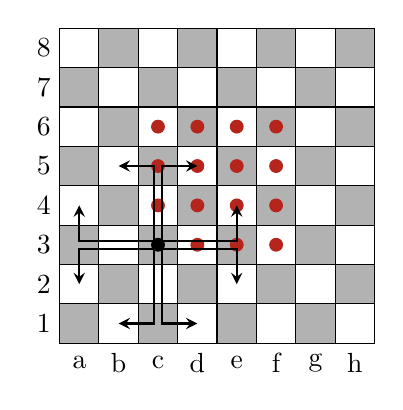
\begin{tikzpicture}[x=5mm,y=5mm]
                \draw[fill=black!30,even odd rule] (0,0) 
                foreach \n in {1,2,3,4} { -- ++ (8,0) -- ++ (0,1) -- ++ (-8,0) -- ++ (0,1) } -- (8,8)
            
                foreach \n in {1,2,3,4} { -- ++ (0,-8) -- ++ (-1,0) -- ++ (0,8) -- ++ (-1,0) } -- cycle
            
                foreach[count=\n] \m in {a,b,...,h} { (-0.4,\n-0.5) node {\n} (\n-0.5,-0.5) node {\m} };

                \fill (2.5,2.5) circle[radius=2.5pt];
                \fill[BrickRed] (3.5,2.5) circle[radius=2.5pt];
                \fill[BrickRed] (4.5,2.5) circle[radius=2.5pt];
                \fill[BrickRed] (5.5,2.5) circle[radius=2.5pt];
                \fill[BrickRed] (2.5,3.5) circle[radius=2.5pt];
                \fill[BrickRed] (3.5,3.5) circle[radius=2.5pt];
                \fill[BrickRed] (4.5,3.5) circle[radius=2.5pt];
                \fill[BrickRed] (5.5,3.5) circle[radius=2.5pt];
                \fill[BrickRed] (2.5,4.5) circle[radius=2.5pt];
                \fill[BrickRed] (3.5,4.5) circle[radius=2.5pt];
                \fill[BrickRed] (4.5,4.5) circle[radius=2.5pt];
                \fill[BrickRed] (5.5,4.5) circle[radius=2.5pt];
                \fill[BrickRed] (2.5,5.5) circle[radius=2.5pt];
                \fill[BrickRed] (3.5,5.5) circle[radius=2.5pt];
                \fill[BrickRed] (4.5,5.5) circle[radius=2.5pt];
                \fill[BrickRed] (5.5,5.5) circle[radius=2.5pt];
                \draw[-stealth, thick] (2.4,2.6) -- (2.4,4.5) -- (1.5,4.5);
                \draw[-stealth, thick] (2.6,2.6) -- (2.6,4.5) -- (3.5,4.5);
                \draw[-stealth, thick] (2.4,2.4) -- (2.4,0.5) -- (1.5,0.5);
                \draw[-stealth, thick] (2.6,2.4) -- (2.6,0.5) -- (3.5,0.5);
                \draw[-stealth, thick] (2.6,2.6) -- (4.5,2.6) -- (4.5,3.5);
                \draw[-stealth, thick] (2.6,2.4) -- (4.5,2.4) -- (4.5,1.5);
                \draw[-stealth, thick] (2.4,2.6) -- (0.5,2.6) -- (0.5,3.5);
                \draw[-stealth, thick] (2.4,2.4) -- (0.5,2.4) -- (0.5,1.5);
            \end{tikzpicture}
        \end{subfigure}

        \caption{Las flechas muestran los posibles movimientos del caballo comenzando en el círculo negro, y los círculos rojos son posiciones con \emph{la misma cantidad de movimientos} ---similares--- a los del círculo negro.}
        \label{fig:caballitos}
    \end{figure}
\end{example}

Hasta el momento hemos obtenido resultados para la existencia y unicidad de las distribuciones estacionarias así como para el comportamiento asintótico de $n^{-1}\sum_{m = 1}^n P_{ij}^m$. Para finalizar las notas, en la siguiente sección estudiaremos el comportamiento de $P_{ij}^n$ para cadenas de Markov irreducibles.